%%%%%%%%%%%%%%%%%%%%%%%%%%%%%%%%%%%%%%%%%
% Beamer Presentation
% LaTeX Template
% Version 1.0 (10/11/12)
%
% This template has been downloaded from:
% http://www.LaTeXTemplates.com
%
% License:
% CC BY-NC-SA 3.0 (http://creativecommons.org/licenses/by-nc-sa/3.0/)
%
%%%%%%%%%%%%%%%%%%%%%%%%%%%%%%%%%%%%%%%%%

%----------------------------------------------------------------------------------------
%	PACKAGES AND THEMES
%----------------------------------------------------------------------------------------

\documentclass[14pt,handout]{beamer}
%%\documentclass[14pt]{beamer}

\mode<presentation> {

% The Beamer class slide themes
\usetheme{Madrid} %i was using this one

% Beamer class color themes

%\usecolortheme{albatross}

%\setbeamertemplate{footline} % To remove the footer line in all slides uncomment this line
%\setbeamertemplate{footline}[page number] % To replace the footer line in all slides with a simple slide count uncomment this line

%\setbeamertemplate{navigation symbols}{} % To remove the navigation symbols from the bottom of all slides uncomment this line
}

\usepackage{graphicx} % Allows including images
\usepackage{booktabs} % Allows the use of \toprule, \midrule and \bottomrule in tables
\usepackage{hyperref}
\usepackage{helvet}
\usepackage[T1]{fontenc}
\usepackage{textcomp}

%----------------------------------------------------------------------------------------
%	TITLE PAGE
%----------------------------------------------------------------------------------------

\title[RNAseq Practical pt3/3]{RNAseq Walkthrough part 3/3} % The short title appears at the bottom of every slide, the full title is only on the title page

\author{C. Ryan Campbell} % Your name
\institute[Duke] % Your institution as it will appear on the bottom of every slide, may be shorthand to save space
{
Duke University \\ % Your institution for the title page
\medskip
\textit{c.ryan.campbell@duke.edu} % Your email address
}
\date{9 Nov 2017} % Date, can be changed to a custom date

\begin{document}

\begin{frame}
\titlepage % Print the title page as the first slide
\end{frame}

\begin{frame}
\frametitle{Overview} % Table of contents slide, comment this block out to remove it
\tableofcontents % Throughout your presentation, if you choose to use \section{} and \subsection{} commands, these will automatically be printed on this slide as an overview of your presentation
\end{frame}

%----------------------------------------------------------------------------------------
%	PRESENTATION SLIDES
%----------------------------------------------------------------------------------------

%------------------------------------------------
\begin{frame}
\frametitle{Today's Goals}
\begin{itemize}
	\item<+-> Discuss Methods and Results
	\item<+-> Format data for DESeq
	\item<+-> Run DESeq
\end{itemize}
\end{frame}


%------------------------------------------------
\section{Methods \& Results}
%------------------------------------------------

%------------------------------------------------
\subsection{Methods}
%------------------------------------------------

%------------------------------------------------
\begin{frame}
\frametitle{Methods}
\begin{itemize}
	\sffamily
	\normalsize
	\item<+-> Should be pretty dry reading
	\item<+-> Read like a lab notebook or recipe
	\item<+-> The reader should be able to replicate your work
\end{itemize}
\end{frame}

%------------------------------------------------
\begin{frame}
\frametitle{Methods}
\begin{itemize}
	\sffamily
	\normalsize
	\item<+-> If you used a software it should be in the Methods
	\item<+-> Include details of usage (flags, settings, or if you used defaults)
	\item<+-> Be sure to cite the software and list the version
\end{itemize}
\end{frame}

%------------------------------------------------
\begin{frame}
\frametitle{Methods}
\begin{center}
	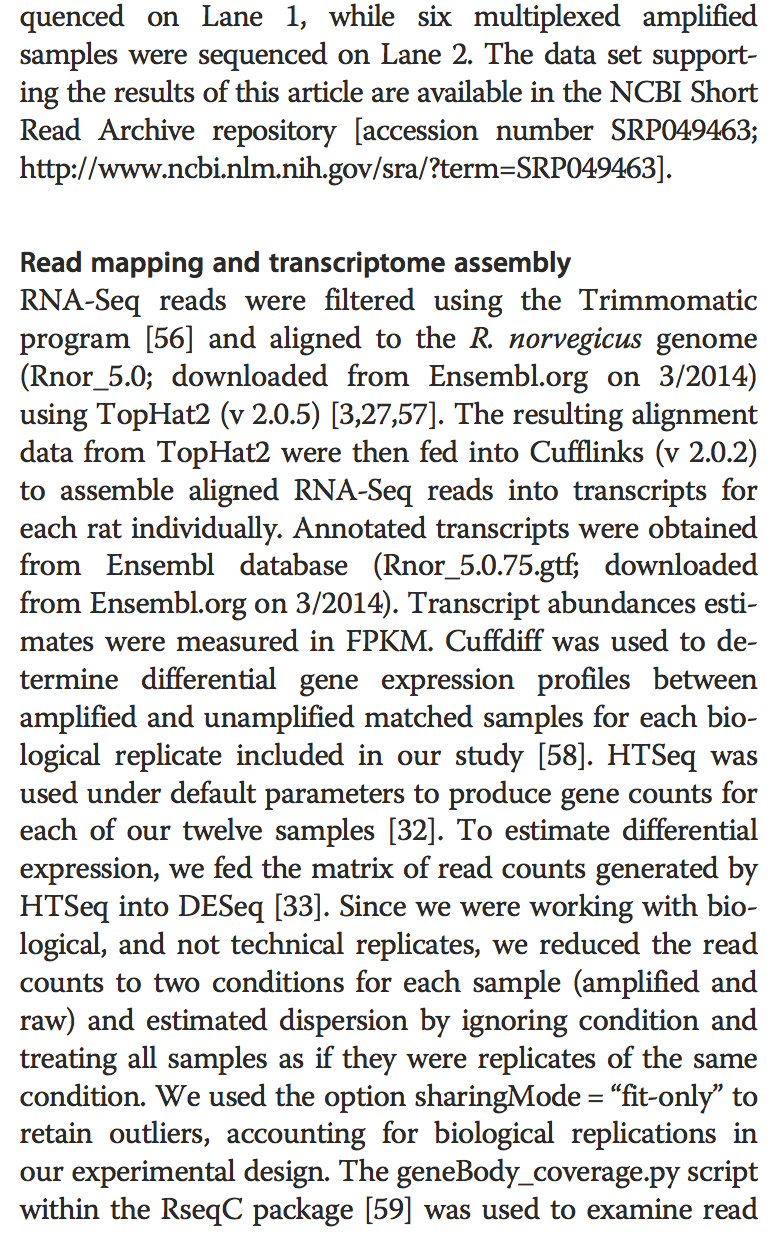
\includegraphics[width=.5\textwidth]{images_20171109_methods.png}
\end{center}
\end{frame}

%------------------------------------------------
\subsection{Results}
%------------------------------------------------

%------------------------------------------------
\begin{frame}
\frametitle{Results}
\begin{itemize}
	\sffamily
	\normalsize
	\item<+-> Less dry reading, still a bit boring
	\item<+-> This is \underline{JUST} for outcomes of the work
	\item<+-> No analysis or interpretation, only what the results were
\end{itemize}
\end{frame}

%------------------------------------------------
\begin{frame}
\frametitle{Results}
\begin{itemize}
	\sffamily
	\normalsize
	\item<+-> If a step was in your Methods, list the results
	\item<+-> This is obvious sometimes:
	\item<+-> "After running trimmomatic n\% of the data was kept"
	\item<+-> And less so others:
	\item<+-> DESeq2 has a lot of output, summarize what is most important
\end{itemize}
\end{frame}

%------------------------------------------------
\begin{frame}
\frametitle{Results}
\begin{center}
	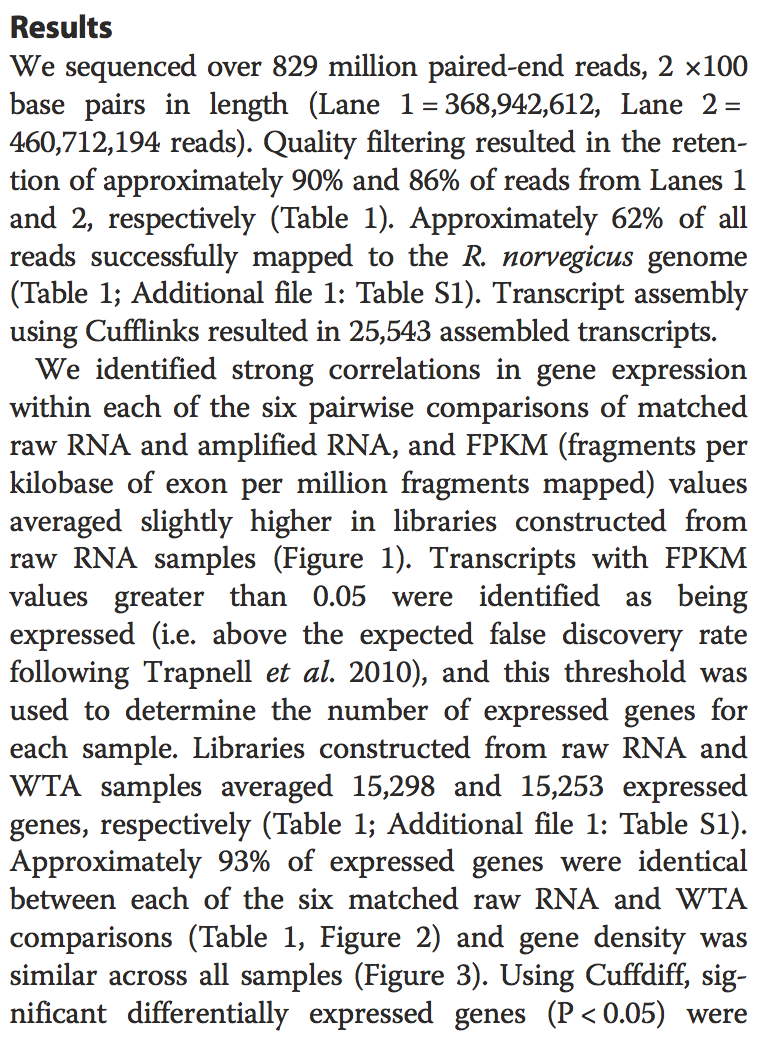
\includegraphics[width=.5\textwidth]{images_20171109_results.png}
\end{center}
\end{frame}

%------------------------------------------------
\begin{frame}
\frametitle{SLURM Interactive Node}
\begin{itemize}
	\footnotesize
	\ttfamily
	\begin{block}{}
	\item[] srun --mem-per-cpu=4000MB --pty bash -i
	\end{block}
	\sffamily
	\normalsize
	\item When you're done with an interactive node type \texttt{exit}
	\item Also, check your SLURM queue \texttt{squeue -u <netID>}
	\item If you're still running a ``bash'' job, use \texttt{scancel <job ID number>} to cancel it
\end{itemize}
\end{frame}

%------------------------------------------------
\section{DESeq2}
%------------------------------------------------

%------------------------------------------------
\subsection{cluster}
%------------------------------------------------

%------------------------------------------------
\begin{frame}
\frametitle{Files to Use}
\begin{itemize}
	\item I have some example files to use for the DESeq tutorial
	\item They're human RNAseq files from a hypoxia experiment:
	\footnotesize
	\ttfamily
	\begin{block}{}
	\item[] ls -lthr /work/cc216/490S/cc216/RNAseq\_pt3
	\end{block}
	\sffamily
\end{itemize}
\end{frame}

%------------------------------------------------
\begin{frame}
\frametitle{Combining htseq Output}
\begin{itemize}
	\item There are four samples of htseq-count output:
	\footnotesize
	\ttfamily
	\begin{block}{}
	\item[] s01.norm.counts, s02.norm.counts, s03.hypo.counts, s04.hypo.counts
	\item[] > head s01.norm.counts
	\item[] 3.8-1.4	0
	\item[] 3.8-1.5	0
	\item[] 5-HT3C2	0
	\item[] A1BG	252
	\item[] A1BG-AS1	47
	\end{block}
	\sffamily
\end{itemize}
\end{frame}

%------------------------------------------------
\begin{frame}
\frametitle{Combining htseq Output}
\begin{itemize}
	\item Use \texttt{paste} to combine these files:
	\footnotesize
	\ttfamily
	\begin{block}{}
	\item[] > paste s01.norm.counts s02.norm.counts s03.hypo.counts s04.hypo.counts
	\item[] 3.8-1.4	0	3.8-1.4	0	3.8-1.4	0	3.8-1.4	0
	\item[] 3.8-1.5	0	3.8-1.5	0	3.8-1.5	0	3.8-1.5	0
	\item[] 5-HT3C2	0	5-HT3C2	0	5-HT3C2	0	5-HT3C2	0
	\item[] A1BG	252	A1BG	192	A1BG	175	A1BG	153
	\item[] A1BG-AS1	47	A1BG-AS1	28	A1BG-AS1	31	A1BG-AS1	35
	\end{block}
	\sffamily
\end{itemize}
\end{frame}

%------------------------------------------------
\begin{frame}
\frametitle{Combining htseq Output}
\begin{itemize}
	\item And \texttt{cut} to eliminate redundant columns:
	\footnotesize
	\ttfamily
	\begin{block}{}
	\item[] > paste s01.norm.counts s02.norm.counts s03.hypo.counts s04.hypo.counts | cut -f1,2,4,6,8
	\item[] 3.8-1.4	0	0	0	0
	\item[] 3.8-1.5	0	0	0	0
	\item[] 5-HT3C2	0	0	0	0
	\item[] A1BG	252	192	175	153
	\item[] A1BG-AS1	47	28	31	35
	\end{block}
	\sffamily
	\item[] Finally write to a file:
	\ttfamily
	\begin{block}{}
	\item[] > paste s01.norm.counts s02.norm.counts s03.hypo.counts s04.hypo.counts | cut -f1,2,4,6,8 > hypoxia\_hsap.counts
	\end{block}
	\sffamily
\end{itemize}
\end{frame}

%------------------------------------------------
\begin{frame}
\frametitle{Move the count table down to your laptop}
\begin{itemize}
	\item[] On your laptop's terminal (not slogin): 
	\footnotesize
	\ttfamily
	\begin{block}{}
	\item[] scp -v <yournetID>@dcc-slogin-02.oit.duke.edu:
	\item[] /work/cc216/490S/cc216/RNAseq\_pt3/*.counts 
	\item[] ~/<your laptop location>/
	\end{block}
	\sffamily
	\item[] (pay attention to the spaces! the spacing above isn't correct because the slide is too narrow)
\end{itemize}
\end{frame}

%------------------------------------------------
\subsection{RStudio}
%------------------------------------------------

%------------------------------------------------
\begin{frame}
\frametitle{DESeq2}
\begin{itemize}
	\item<+-> See the website for installation instructions
	\item<+-> Needs two things:
	\begin{enumerate}
	\item<+-> A matrix of counts = ``cts''
	\item<+-> A matrix of sample conditions = ``coldata''
	\end{enumerate}
\end{itemize}
\end{frame}

%------------------------------------------------
\begin{frame}
\frametitle{DESeq2}
\begin{itemize}
	\item[] In R: 
	\footnotesize
	\ttfamily
	\begin{block}{}
	\item[] > head(cts, n = 4)
	\item[]         s01norm s02norm s03hypox s04hypox
	\item[] 3.8-1.4       0       0        0        0
	\item[] 3.8-1.5       0       0        0        0
	\item[] 5-HT3C2       0       0        0        0
	\item[] A1BG        252     192      175      153 
	\item[]
	\item[] > coldata
	\item[]          condition   type        
	\item[] s01norm  "untreated" "paired-end"
	\item[] s02norm  "untreated" "paired-end"
	\item[] s03hypox "treated"   "paired-end"
	\item[] s04hypox "treated"   "paired-end" 
	\end{block}
	\sffamily
\end{itemize}
\end{frame}

%------------------------------------------------
\begin{frame}
\frametitle{DESeq2}
\begin{itemize}
	\item Order must match (01, 02, 03...)
	\item Name the columns and rows appropriately 
	\footnotesize
	\ttfamily
	\begin{block}{}
	\item[] > rownames(coldata)
	\item[] [1] "s01norm"  "s02norm"  "s03hypox" "s04hypox"
	\item[] 
	\item[] > colnames(coldata)
	\item[] [1] "condition" "type"
	\end{block}
	\sffamily
	\item[] You use the same function to call (see above) define (see below) column and row names:
	\ttfamily
	\footnotesize
	\begin{block}{}
	\item[] > colnames(coldata) <- c("condition","type")
	\end{block}
\end{itemize}
\end{frame}

%------------------------------------------------
\begin{frame}
\frametitle{DESeq2}
\begin{itemize}
	\item Get your data in this format
	\item Keep track of your work in a .Rmd file!!
	\item Then (and only then) proceed to running DESeq (see further slides)
\end{itemize}
\end{frame}

%------------------------------------------------
\begin{frame}
\frametitle{DESeq2 Formatting Tips: Reading Data}
\begin{itemize}
	\item In R:
	\footnotesize
	\ttfamily
	\begin{block}{}
	\item[] > countfile <- read.table("hypoxia\_hsap.counts")
	\item[] > head(countfile, n = 5)
	\item[]        V1  V2  V3  V4  V5
	\item[] 1 3.8-1.4   0   0   0   0
	\item[] 2 3.8-1.5   0   0   0   0
	\item[] 3 5-HT3C2   0   0   0   0
	\item[] 4    A1BG 252 192 175 153
	\end{block}
	\sffamily
	\item[] Now we need to get the data into matrices with the correct row and column names
\end{itemize}
\end{frame}

%------------------------------------------------
\begin{frame}
\frametitle{DESeq2 Formatting Tips: Transforming Data}
\begin{itemize}
	\item \texttt{countfile} contains the count data
	\item We need to format it appropriately 
	\footnotesize
	\ttfamily
	\begin{block}{}
	\item[] > cts <- as.matrix(countfile[,2:5])
	\item[] > colnames(cts) <- c("s01norm","s02norm","s03hypox","s04hypox")
	\item[] > rownames(cts) <- countfile[,1]
	\item[] > head(cts, n = 4)
	\item[]        s01norm s02norm s03hypox s04hypox
	\item[] 3.8-1.4       0       0        0        0
	\item[] 3.8-1.5       0       0        0        0
	\item[] 5-HT3C2       0       0        0        0
	\item[] A1BG        252     192      175      153 
	\end{block}
	\sffamily
	\item[] First take in only the data (columns 2-5) as a matrix
	\item[] Then name the columns the sample IDs
	\item[] And the rows the geneIDs
\end{itemize}
\end{frame}

%------------------------------------------------
\begin{frame}
\frametitle{DESeq2 Formatting: coldata matrix}
\begin{itemize}
	\item<+-> \texttt{coldata} needs to contain the appropriate sample info
	\item<+-> Each row is a sample, each column is information about the sample
	\item<+-> Experimental Treatment, Read Format, Cell Type can all be pertinent info
	\item<+-> First we will make a vector with the information
	\item<+-> Then we'll take the data and make it into a 2x4 matrix
\end{itemize}
\end{frame}

%------------------------------------------------
\begin{frame}
\frametitle{DESeq2 Formatting: coldata matrix}
\begin{itemize}
	\ttfamily
	\footnotesize
	\begin{block}{}
	\item[] > sampleinfo <- c("untreated","untreated","treated","treated",
	\item[]     "paired-end","paired-end","paired-end","paired-end")
	\item[] > sampleinfo
	\item[] [1] "untreated"  "untreated"  "treated"    "treated"    "paired-end" "paired-end"
	\item[] [7] "paired-end" "paired-end" 
	\item[] > coldata <- matrix(sampleinfo, nrow = 4, ncol = 2, byrow = F)
	\item[] > coldata
	\item[]      [,1]        [,2]        
	\item[] [1,] "untreated" "paired-end"
	\item[] [2,] "untreated" "paired-end"
	\item[] [3,] "treated"   "paired-end" 
	\item[] [4,] "treated"   "paired-end" 
	\end{block}
	\sffamily
\end{itemize}
\end{frame}

%------------------------------------------------
\begin{frame}
\frametitle{DESeq2 Formatting: coldata matrix}
\begin{itemize}
	\item<+-> \texttt{coldata} now needs correct row and column names
	\item<+-> What should they be? (hint: it is in this slide deck)
	\item<+-> Once you decide, use \texttt{rownames()} and \texttt{colnames()} to add them
\end{itemize}
\end{frame}


%------------------------------------------------
\begin{frame}
\frametitle{Today's (Remaining) Goals}
\large
\begin{enumerate}
	\item<+-> Format data for DESeq
	\item<+-> Successfully run DESeq
\end{enumerate}
\end{frame}

%------------------------------------------------
\section{Running DESeq2}
%------------------------------------------------

%------------------------------------------------
\begin{frame}
\frametitle{DESeq2 guides}
\begin{itemize}
	\item Here are the DESeq guides that I have summarized in this walkthrough:
	\item \href{http://bioconductor.org/packages/devel/bioc/vignettes/DESeq2/inst/doc/DESeq2.html}{Walkthrough Link}
	\item Focus on ``Quick Start'' and more specifically:
	\item Setting the R objects \texttt{cts} and \texttt{coldata} correctly
	\item Using \texttt{paste} (a unix command) to format your data into \texttt{cts}
	\footnotesize
	\item[] http://bioconductor.org/packages/devel/bioc/vignettes/
	\item[] DESeq2/inst/doc/DESeq2.html
\end{itemize}
\end{frame}

%------------------------------------------------
\begin{frame}
\frametitle{DESeq2}
\begin{itemize}
	\item To run DESeq, first create a ``DESeq dataset''
	\footnotesize
	\ttfamily
	\begin{block}{}
	\item[] > dds <- DESeqDataSetFromMatrix(countData = cts,
    \item[]                          colData = coldata,
    \item[]                          design = \url{~} condition)
    \item[]
	\item[] > dds
	\end{block}
	\sffamily
	\item[] Where cts and coldata are the files described earlier
	\item[] Output: 
	\ttfamily
	\footnotesize
	\begin{block}{}
	\item[] class: DESeqDataSet 
	\item[] dim: 45381 4 
	\item[] metadata(1): version
	\end{block}
\end{itemize}
\end{frame}

%------------------------------------------------
\begin{frame}
\frametitle{DESeq2}
\begin{itemize}
	\item Let's throw out genes with low expression levels (here, below 10)
	\footnotesize
	\ttfamily
	\begin{block}{}
	\item[] > keep <- rowSums(counts(dds)) >= 10
	\item[] > dds <- dds[keep,]
	\item[] > dds\$condition <- relevel(dds\$condition, ref = "untreated")
	\item[] > dds
	\end{block}
	\sffamily
	\item[] Output: 
	\ttfamily
	\footnotesize
	\begin{block}{}
	\item[] class: DESeqDataSet 
	\item[] dim: 17380 4 
	\item[] metadata(1): version
	\end{block}
	\sffamily
	\item[] We've shrunk our gene list by roughly 60 percent 
\end{itemize}
\end{frame}

%------------------------------------------------
\begin{frame}
\frametitle{DESeq2}
\begin{itemize}
	\item Now... Run DESeq!!!
	\footnotesize
	\ttfamily
	\begin{block}{}
	\item[] > dds <- DESeq(dds)
	\item[] > res <- results(dds)
	\item[] > res
	\end{block}
	\sffamily
	\item[] Output: 
	\ttfamily
	\tiny
	\begin{block}{}
	\item[] log2 fold change (MAP): condition treated vs untreated 
	\item[] Wald test p-value: condition treated vs untreated 
	\item[] DataFrame with 17380 rows and 6 columns
	\item[]                            baseMean log2FoldChange      lfcSE        stat       pvalue
	\item[]                           <numeric>      <numeric>  <numeric>   <numeric>    <numeric>
	\item[] A1BG                     189.927175    -0.20541335 0.16773404 -1.22463727    0.2207119
	\item[] A1BG-AS1                  34.902293     0.02668120 0.26939459  0.09904134    0.9211054
	\end{block}
	\sffamily
\end{itemize}
\end{frame}

%------------------------------------------------
\begin{frame}
\frametitle{DESeq2}
\begin{itemize}
	\item A few final things to do and explore:
	\item[] 
	\item Sort the results by p-value
	\footnotesize
	\ttfamily
	\begin{block}{}
	\item[] > resOrdered <- res[order(res\$pvalue),]
	\end{block}
	\sffamily
	\item Summarize the results
	\footnotesize
	\ttfamily
	\begin{block}{}
	\item[] > summary(res)
	\end{block}
	\sffamily
	\item How many genes are significant (at 0.10 and 0.05)?
	\footnotesize
	\ttfamily
	\begin{block}{}
	\item[] > sum(res\$padj < 0.1, na.rm=TRUE)
	\item[] > sum(res\$padj < 0.05, na.rm=TRUE)
	\end{block}
	\sffamily

\end{itemize}
\end{frame}

%------------------------------------------------
\begin{frame}
\frametitle{Plotting in DESeq2}
\begin{itemize}
	\item There are several ways to plot this data
	\item[] 
	\item You can used the built-in DESeq functions:
	\footnotesize
	\ttfamily
	\begin{block}{}
	\item[] > plotMA(res, ylim=c(-2,2))
	\item[]
	\item[] > plotCounts(dds, gene=which.min(res\$padj), intgroup="condition") 
	\end{block}
	\sffamily
	\item Or the R plotting function:
	\footnotesize
	\ttfamily
	\begin{block}{}
	\item[] > plot(res\$log2FoldChange,-log(res\$padj))
	\end{block}
\end{itemize}
\end{frame}

%------------------------------------------------
\begin{frame}
\frametitle{Plotting in DESeq2}
\begin{itemize}
	\ttfamily
	\begin{block}{}
	\item[] > plotMA(res, ylim=c(-2,2))
	\end{block}
	\begin{center}
	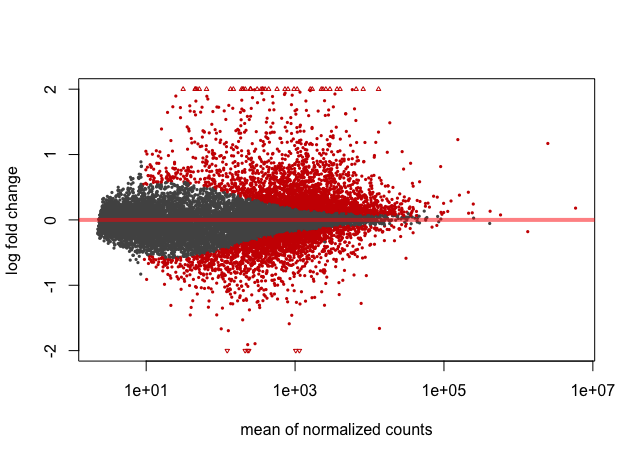
\includegraphics[width=.8\textwidth]{images_20171109_plotMA.png}
	\end{center}
\end{itemize}
\end{frame}

%------------------------------------------------
\begin{frame}
\frametitle{Plotting in DESeq2}
\begin{itemize}
	\ttfamily
	\begin{block}{}
	\item[] > plotCounts(dds, gene=which.min(res\$padj), intgroup="condition") 
	\end{block}
	\begin{center}
	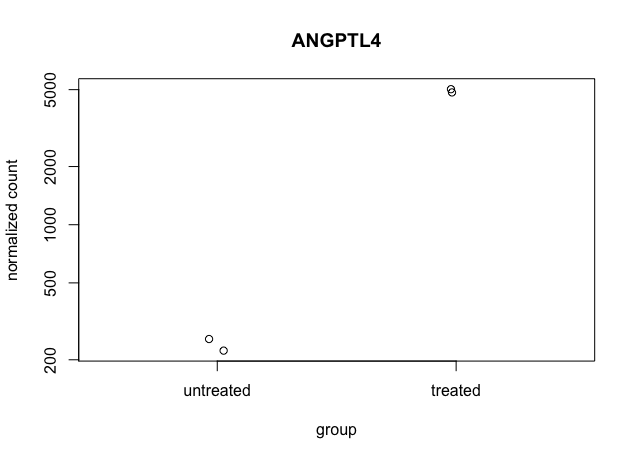
\includegraphics[width=.8\textwidth]{images_20171109_plotCounts.png}
	\end{center}
\end{itemize}
\end{frame}

%------------------------------------------------
\begin{frame}
\frametitle{Plotting in DESeq2}
\begin{itemize}
	\ttfamily
	\begin{block}{}
	\item[] > plot(res\$log2FoldChange,-log(res\$padj))
	\end{block}
	\begin{center}
	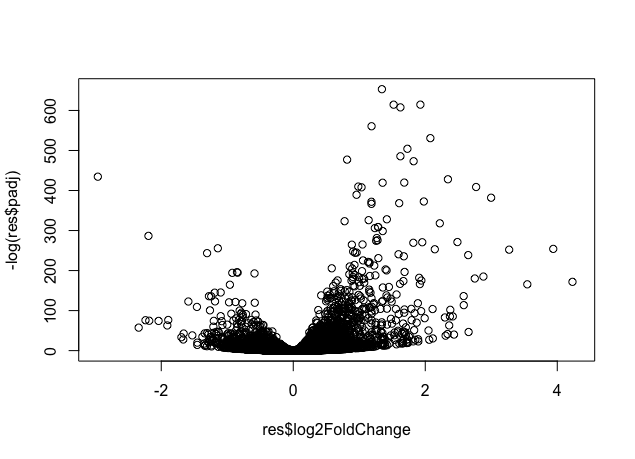
\includegraphics[width=.8\textwidth]{images_20171109_plot.png}
	\end{center}
\end{itemize}
\end{frame}



%------------------------------------------------
\begin{frame}
\Huge{\centerline{The End}}
\end{frame}

%----------------------------------------------------------------------------------------

\end{document} 